\documentclass[11pt]{article}
\usepackage[margin=0.55in]{geometry}
\usepackage{amsmath,amssymb}
\usepackage{lmodern}
\usepackage{xcolor}
\usepackage{tikz}
\pagestyle{empty}
\setlength{\parindent}{0pt}

\definecolor{accent}{HTML}{C2410C}

% One card: \flashcard{col}{row}{topic}{question}
\newcommand{\flashcard}[4]{%
  \begin{scope}[shift={(#1*8.6, -#2*5.6)}]
    \draw[dashed, accent!60, line width=0.5pt, rounded corners=2mm]
      (0,0) rectangle (8.2, -5.2);
    \node[anchor=north west, font=\footnotesize\bfseries, text=accent]
      at (0.35, -0.3) {#3};
    \draw[accent!30, line width=0.4pt] (0.35, -0.85) -- (7.85, -0.85);
    \node[anchor=north west, text width=7.4cm, align=left]
      at (0.35, -1.15) {#4};
    \node[anchor=south east, font=\tiny, text=black!45] at (7.95, -5.05) {front};
  \end{scope}}

\begin{document}

\begin{center}
  {\large\bfseries\color{accent} Calculus I Flashcards, Set 2: Derivatives}\\[2pt]
  {\small Print single sided, cut along the dashed lines, quiz yourself.}
\end{center}

\vspace{0.4em}
\begin{center}
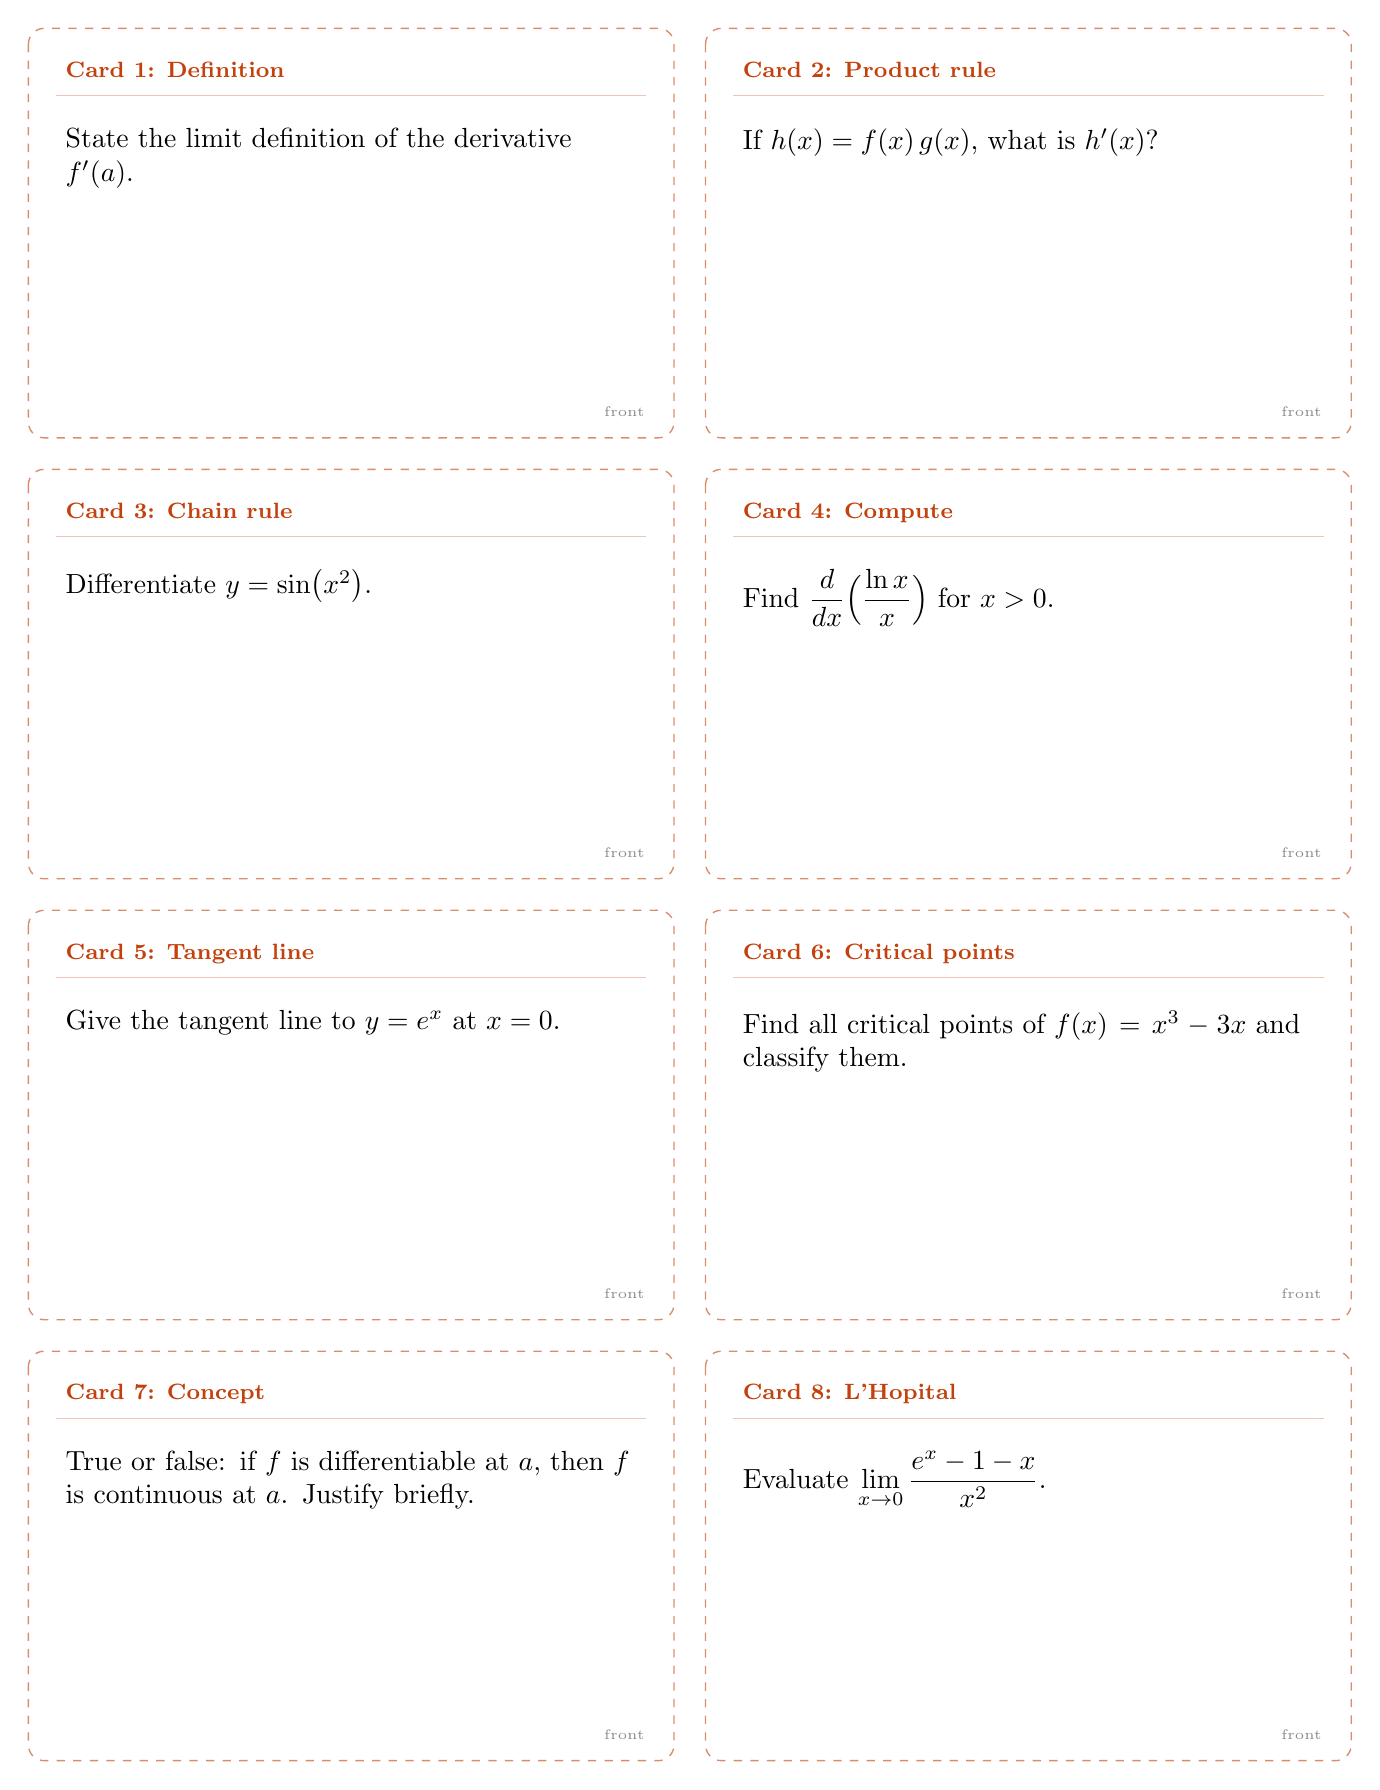
\begin{tikzpicture}[x=1cm, y=1cm]

\flashcard{0}{0}{Card 1: Definition}
  {State the limit definition of the derivative $f'(a)$.}

\flashcard{1}{0}{Card 2: Product rule}
  {If $h(x) = f(x)\,g(x)$, what is $h'(x)$?}

\flashcard{0}{1}{Card 3: Chain rule}
  {Differentiate $y = \sin\bigl(x^2\bigr)$.}

\flashcard{1}{1}{Card 4: Compute}
  {Find $\dfrac{d}{dx}\Bigl(\dfrac{\ln x}{x}\Bigr)$ for $x > 0$.}

\flashcard{0}{2}{Card 5: Tangent line}
  {Give the tangent line to $y = e^{x}$ at $x = 0$.}

\flashcard{1}{2}{Card 6: Critical points}
  {Find all critical points of $f(x) = x^3 - 3x$ and classify them.}

\flashcard{0}{3}{Card 7: Concept}
  {True or false: if $f$ is differentiable at $a$, then $f$ is continuous
   at $a$. Justify briefly.}

\flashcard{1}{3}{Card 8: L'Hopital}
  {Evaluate $\displaystyle\lim_{x \to 0} \frac{e^{x} - 1 - x}{x^2}$.}

\end{tikzpicture}
\end{center}

\end{document}
